\chapter{LANDASAN TEORI}

%------------------------------------------------------------------------------
% Android
%------------------------------------------------------------------------------
\section{Android}
Android adalah sistem operasi berbasis Linux yang dirancang untuk perangkat bergerak seperti ponsel cerdas dan tablet. Aplikasi untuk perangkat Android dapat diporgram dengan Android Software Development Kit (SDK). Kebanyakan perangkat Android saat ini telah dilengkapi dengan berbagai macam sensor, termasuk akselerometer dan giroskop. Sensor-sensor ini dapat diakses melalui \textit{Application Programming Interface (API)} yang telah tersedia dalam Android SDK\@. Gambar~\ref{gambar:koordinat-sensor-android} menunjukkan sistem koordinat sensor-sensor relatif terhadap perangkat yang digunakan dalam Android SDK\@.

\begin{figure}[h!]
    \centering
    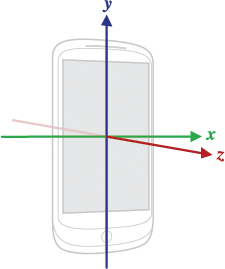
\includegraphics[width=5cm]{gambar/landasan-teori/axis_device.png}
    \caption{Sistem koordinat relatif terhadap perangkat yang digunakan dalam Android SDK (developer.android.com)}
    \label{gambar:koordinat-sensor-android}
\end{figure}

Sensor pada Android dapat diakses dengan membuat \mintinline{java}{SensorManager} yang diinisialisasi dengan \mintinline{java}{getSystemService(Context.SENSOR_SERVICE)}, seperti contoh pada Gambar~\ref{listing:teori-inisialisasi-sensormanager}.

\begin{figure}[h]
    \begin{minted}{java}
        private SensorManager mSensorManager;
        private Sensor sensor;

        mSensorManager = (SensorManager)
        getSystemService(Context.SENSOR_SERVICE)
        sensor = mSensorManager.getDefaultSensor(JENIS_SENSOR)
    \end{minted}
    \caption{Inisialisasi \textit{SensorManager}}
    \label{listing:teori-inisialisasi-sensormanager}
\end{figure}


%------------------------------------------------------------------------------
% Akselerometer
%------------------------------------------------------------------------------
\section{Akselerometer}
Akselerometer adalah sensor yang digunakan untuk mengukur percepatan. Pada akselerometer \textit{Microelectrochemical System (MEMS)}, percepatan diukur dengan mengaitkan massa pada pegas dan melihat penyimpangan massa dari posisi setimbangnya \Parencite{milette-2012}, seperti yang diilustrasikan pada Gambar~\ref{gambar:akselerometer-mems}.

\begin{figure}[h!]
    \centering
    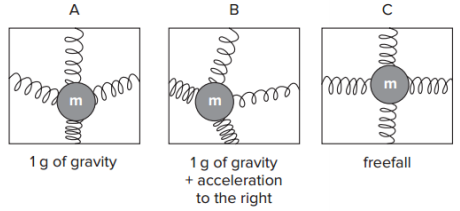
\includegraphics[width=10cm]{gambar/landasan-teori/akselerometer-mems.png}
    \caption{Gaya dikenakan pada massa yang terikat pada pegas \Parencite{milette-2012}}
    \label{gambar:akselerometer-mems}
\end{figure}

Pada sistem operasi Android, sensor akselerometer dapat diakses dengan menggunakan argumen \mintinline{java}{Sensor.TYPE_ACCELEROMETER} pada metode \mintinline{java}{getDefaultSensor()}, seperti contoh pada Gambar~\ref{listing:teori-akses-akselerometer}.

\begin{figure}[h]
    \begin{minted}{java}
        private SensorManager mSensorManager;
        private Sensor accelerometer;

        mSensorManager = (SensorManager)
        getSystemService(Context.SENSOR_SERVICE)
        sensor = mSensorManager.getDefaultSensor(Sensor.TYPE_ACCELEROMETER)
    \end{minted}
    \caption{Akses sensor akselerometer pada Android}
    \label{listing:teori-akses-akselerometer}
\end{figure}

Data bacaan sensor disimpan dalam larik multidimensi pada \mintinline{java}{SensorEvent}. Data tersebut dapat dibaca dengan mengimplementasikan metode \textit{callback} \linebreak \mintinline{java}{onSensorChanged(SensorEvent event)}. Nilai bacaan sumbu x, y dan z akselerometer dapat diambil secara berurutan pada larik \mintinline{java}{SensorEvent.values} dengan indeks nol, satu dan dua. Gambar~\ref{listing:teori-pengambilan-data-sensor} menunjukkan contoh pengambilan data sensor akselerometer.

\begin{figure}[h]
    \begin{minted}{java}
        public void onSensorChanged(SensorEvent event) {
            ax = event.values[0]
            ay = event.values[1]
            az = event.values[2]
        }
    \end{minted}
    \caption{Pengambilan data sensor pada Android}
    \label{listing:teori-pengambilan-data-sensor}
\end{figure}



%------------------------------------------------------------------------------
% Giroskop
%------------------------------------------------------------------------------
\section{Giroskop}
Seperti akselerometer MEMS, giroskop MEMS juga merupakan massa yang dikaitkan pada pegas. Giroskop MEMS digunakan untuk mengukur gaya coriolis yang terjadi karena rotasi. Giroskop MEMS bekerja dengan mendorong massa bolak-balik dalam satu sumbu. Ketika giroskop berputar, gaya coriolis membuat massa menyimpang dari arah getarannya sehingga bergerak ke arah sumbu yang berbeda. Pergerakan ini diukur secara elektrik dengan plat kapasitor, satu plat ditempatkan pada kerangka dan satu plat pada massa yang bergerak. Gaya coriolis hanya berlaku ketika perangkat berputar, sehingga giroskop dapat digunakan untuk mengukur kecepatan sudutnya \Parencite{milette-2012}.

Pada sistem operasi Android, sensor giroskop dapat diakses dengan menggunakan argumen \mintinline{java}{Sensor.TYPE_GYROSCOPE} pada metode \mintinline{java}{getDefaultSensor()}, seperti contoh pada Gambar~\ref{listing:teori-akses-giroskop}.

\begin{figure}[h]
    \begin{minted}{java}
        private SensorManager mSensorManager;
        private Sensor accelerometer;

        mSensorManager = (SensorManager)
        getSystemService(Context.SENSOR_SERVICE)
        sensor = mSensorManager.getDefaultSensor(Sensor.TYPE_GYROSCOPE)
    \end{minted}
    \caption{Akses sensor giroskop pada Android}
    \label{listing:teori-akses-giroskop}
\end{figure}

Seperti pada akselerometer, data bacaan sensor disimpan dalam larik multidimensi pada \mintinline{java}{SensorEvent}. Nilai bacaan sumbu x, y dan z giroskop dapat diambil secara berurutan pada larik \mintinline{java}{SensorEvent.values} dengan indeks nol, satu dan dua.


%------------------------------------------------------------------------------
% Deep Learning
%------------------------------------------------------------------------------
\section{Deep Learning}
Pembelajaran mesin adalah kemampuan komputer untuk beradaptasi dengan keadaan baru dan mendeteksi serta meramalkan kemungkinan pola \Parencite{Russell:2009:AIM:1671238}. Dalam pembelajaran mesin, performa suatu algoritma sangat bergantung pada representasi dari data yang digunakan. Setiap informasi yang menjadi representasi data disebut sebagai fitur.

Salah satu masalah dalam pembelajaran mesin adalah sulitnya mengetahui fitur-fitur apa saja yang harus diekstrak dari suatu set data. Masalah ini dapat diatasi dengan menggunakan pembelajaran mesin bukan hanya untuk menemukan pemetaan dari representasi ke output, tapi juga menemukan representasi itu sendiri. Pendekatan ini dikenal dengan \textit{representation learning} \Parencite{Goodfellow-2016}.

Pada aplikasinya di dunia nyata, \textit{representation learning} sering mengalami kesulitan dalam menemukan representasi dari data yang kompleks. \textit{Deep learning} mengatasi masalah ini dengan membuat representasi yang disusun oleh representasi-representasi lain yang lebih sederhana.

\citeauthor{Goodfellow-2016} mendefinisikan \textit{deep learning} sebagai salah satu jenis pembelajaran mesin yang memiliki kemampuan dan fleksibilitas tinggi dengan belajar merepresentasikan dunia sebagai hierarki konsep yang bersarang. Setiap konsep didefinisikan oleh kaitannya terhadap konsep-konsep yang lebih sederhana dan representasi yang lebih abstrak dihitung berdasarkan representasi yang kurang abstrak. Perbandingan \textit{deep learning} dengan sistem inteligensia buatan lainnya dapat dilihat pada Gambar~\ref{gambar:perbandingan-ai}.

\begin{figure}
    \centering
    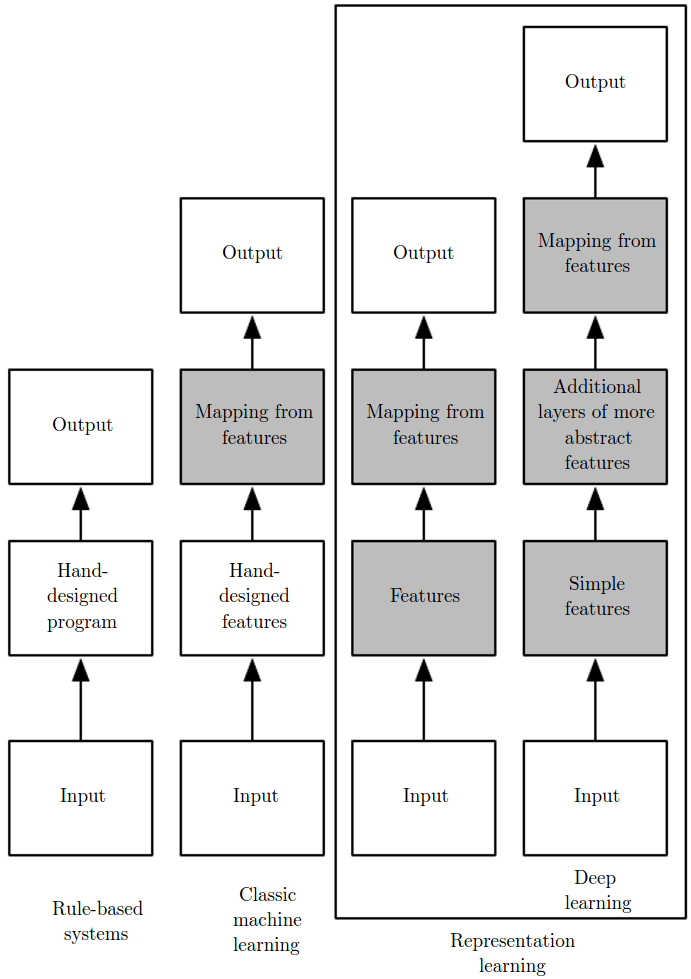
\includegraphics[width=12cm]{gambar/landasan-teori/perbandingan-ai.png}
    \caption{Perbandingan sistem AI. Kotak berwarna abu-abu menunjukkan komponen yang dapat belajar dari data \Parencite{Goodfellow-2016}}
    \label{gambar:perbandingan-ai}
\end{figure}


%------------------------------------------------------------------------------
% Convolutional Neural Network
%
% TODO:
% - Apa perlu membahas sparse interactions, paramater sharing dan
%   equivariant representations?
% - Terjemahan paragraf pertama
%
%------------------------------------------------------------------------------
\section{Convolutional Neural Network}
Convolutional Neural Network (CNN) adalah jenis jaringan saraf untuk mengolah data dengan topologi berbentuk \textit{grid}, seperti data \textit{time-series} yang dapat dianggap sebagai \textit{grid} 1D dengan sample pada interval tertentu, dan data citra yang dapat dianggap sebagai \textit{grid} 2D dari pixel. CNN menggunakan operasi konvolusi untuk menggantikan operasi perkalian matriks pada setidaknya satu lapisan \Parencite{Goodfellow-2016}. Operasi konvolusi dinotasikan sebagai:

\begin{equation}
    \label{eq:konvolusi}
    s(i) = (x * w)(i)
\end{equation}

Dalam terminologi CNN $x$ merupakan input, $w$ adalah kernel, dan outputnya disebut sebagai \textit{feature map}. Input $x$ merupakan larik multidimensi (tensor) parameter yang disesuaikan oleh algoritma pembelajaran.

Saat bekerja dengan data diskrit, persamaan~\ref{eq:konvolusi} dapat ditulis sebagai persamaan konvolusi diskrit:

\begin{equation}
    \label{eq:konvolusi-diskrit}
    s(i) = (x * w)(i) = \sum_{a=-\infty}^{\infty} x(a) w(i - a)
\end{equation}

Pada umumnya, konvolusi digunakan pada lebih dari satu sumbu. Misalnya, jika input adalah data dua dimensi seperti pada Gambar~\ref{gambar:konvolusi-2d}, maka digunakan kernel dua dimensi:
\begin{equation}
    \label{eq:konvolusi-2d}
    S(i,j) = (I * K)(i,j) = \sum_{m}\sum_{n}I(m,n)K(i-m, j-n)
\end{equation}

\begin{figure}[t!]
    \centering
    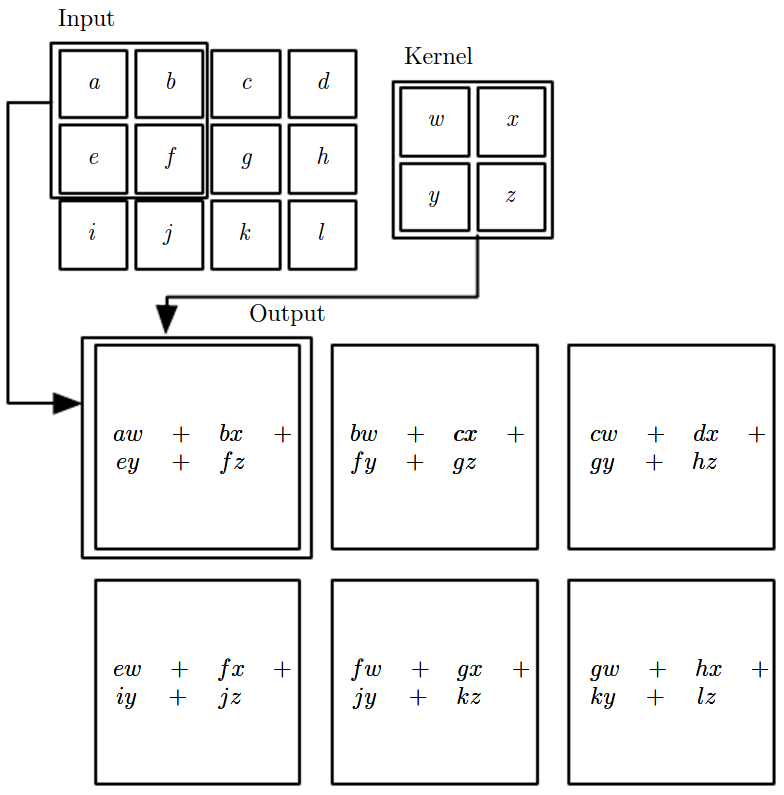
\includegraphics[width=10cm]{gambar/landasan-teori/konvolusi-2d.png}
    \caption{Contoh operasi konvolusi pada data dua dimensi \Parencite{Goodfellow-2016}}
    \label{gambar:konvolusi-2d}
\end{figure}


%------------------------------------------------------------------------------
% Recurrent Neural Network
%
% TODO:
% - Ganti gambar RNN
%------------------------------------------------------------------------------
\section{Recurrent Neural Network}
Recurrent Neural Network (RNN) adalah keluarga jaringan saraf untuk memproses data sekuensial. RNN merupakan \textit{feedforward neural network} dengan hubungan yang berputar. Gambar~\ref{gambar:rnn} menunjukkan graf RNN dan graf yang setara namun telah dibentangkan untuk setiap langkah waktu. RNN dapat memetakan riwayat dari input sebelumnya ke setiap output. Dengan kata lain, koneksi yang berulang ini memungkinkan memori dari input sebelumnya tersimpan dalam kondisi internal jaringan, sehingga mempengaruhi output~\Parencite{graves-2012}.

\begin{figure}
    \centering
    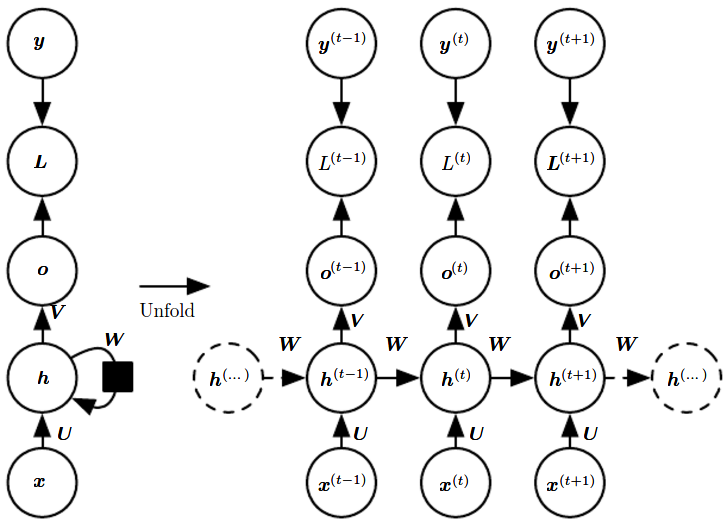
\includegraphics[width=10cm]{gambar/landasan-teori/rnn.png}
    \caption{Graf komputasi \textit{recurrent neural network} \Parencite{Goodfellow-2016}}
    \label{gambar:rnn}
\end{figure}


%------------------------------------------------------------------------------
% Long Short-Term Memory
%------------------------------------------------------------------------------
\section{Long Short-Term Memory}
Long Short-Term Memory (LSTM) adalah salah satu jenis RNN bergerbang. Arsitektur LSTM terdiri dari kumpulan jaringan dengan hubungan internal berulang yang disebut dengan blok memori. Setiap blok memiliki satu atau lebih sel memori \textit{self-loop} dan tiga unit pengali, yaitu gerbang \textit{input, output} dan \textit{forget} \Parencite{graves-2012}.

\begin{figure}
    \centering
    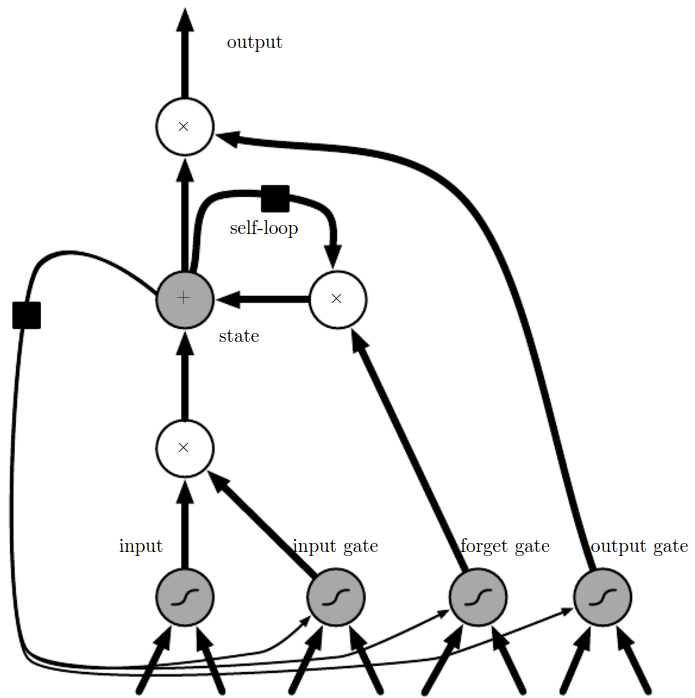
\includegraphics[width=10cm]{gambar/landasan-teori/lstm.png}
    \caption{Graf komputasi sel LSTM \Parencite{Goodfellow-2016}}
    \label{gambar:lstm}
\end{figure}

Pada LSTM, bobot \textit{self-loop} dikendalikan oleh unit gerbang \textit{forget} $f_{i}^{(t)}$ (untuk langkah waktu $t$ dan sel $i$) yang memberikan nilai bobot antara 0 dan 1 melalui unit sigmoid:

\begin{equation}
    f_{i}^{(t)} = \sigma\left(b_{i}^{f} + \sum_{j} U_{i,j}^{f} x_{j}^{(t)} + \sum_{j} W_{i,j}^{f} h_{j}^{(t-1)}\right)
\end{equation}

\noindent
dengan $\pmb{x}^{(t)}$ vektor input saat ini, $\pmb{h}^{(t)}$ vektor \textit{hidden layer} saat ini yang berisi output dari seluruh sel LSTM, dan $\pmb{b}^{f}$, $\pmb{U}^{f}$, $\pmb{W}^{f}$ adalah bias, bobot input dan bobot pengulangan untuk gerbang \textit{forget}. Kondisi internal sel LSTM $s_{i}^{(t)}$ diperbarui sebagai berikut:

\begin{equation}
    s_{i}^{(t)} = f_{i}^{(t)}  s_{i}^{(t-1)} + g_{i}^{(t)} \sigma\left(b_{i} + \sum_{j} U_{i,j} x_{j}^{(t)} + \sum_{j} W_{i,j} h_{j}^{(t-1)} \right)
\end{equation}

\noindent
dengan $\pmb{b}, \pmb{U}$ dan $\pmb{W}$ sebagai bias, bobot input dan bobot pengulangan ke sel LSTM\@. Unit gerbang input eksternal $g_{i}^{(t)}$ dihitung dengan:

\begin{equation}
    g_{i}^{(t)} = \sigma\left(b_{i}^{g} + \sum_{j} U_{i,j}^{g} x_{j}^{(t)} + \sum_{j} W_{i,j}^{g} h_{j}^{(t-1)}\right)
\end{equation}

Output LSTM $h_{i}^{(t)}$ dapat dimatikan melalui gerbang output $q_{i}^{(t)}$, yang juga menggunakan unit sigmoid:

\begin{align}
    \label{eq:output-lstm}
    h_{i}^{(t)} &= \tanh\left(s_{i}^{(t)}\right) q_{i}{(t)} \\
    q_{i}^{(t)} &= \sigma\left(b_{i}^{o} + \sum_{j} U_{i,j}^{o} x_{j}^{(t)} + \sum_{j} W_{i,j}^{o} h_{j}^{(t-1)} \right)
\end{align}

\noindent
dengan $\pmb{b}^{o}, \pmb{U}^{o}$ dan $\pmb{W}^{o}$ sebagai bias, bobot input dan bobot pengulangan \Parencite{Goodfellow-2016}.


%------------------------------------------------------------------------------
% Dropout
%------------------------------------------------------------------------------
\section{Dropout}
Salah satu masalah utama dalam pembelajaran mesin adalah membuat algoritme yang bekerja dengan baik bukan hanya pada data latih, namun juga pada masukan baru. Regularisasi adalah strategi-strategi yang didesain untuk mengurangi error pada pengujian~\Parencite{Goodfellow-2016}.

Dropout merupakan salah satu metode regularisasi yang bekerja dengan baik tanpa membutuhkan komputasi yang tinggi. Dropout melatih kelompok jaringan yang dibentuk dengan menghilangkan unit non-output dari jaringan dasarnya (Gambar~\ref{gambar:dropout}). Setiap kali sampel dimuat ke dalam minibatch, sebuah \textit{binary mask} dibuat secara acak untuk dikenakan pada seluruh input dan hidden unit pada jaringan. Peluang \textit{mask} bernilai satu (menyebabkan unit untuk dimasukkan ke dalam jaringan) didefinisikan sebagai hyperparameter sebelum pelatihan dimulai.

\begin{figure}[h]
    \centering
    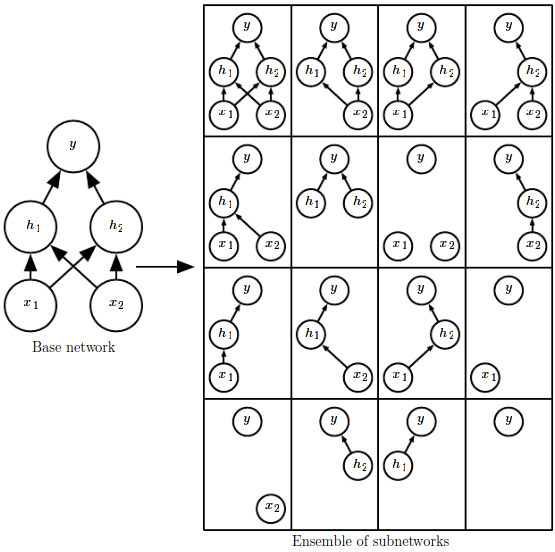
\includegraphics[width=10cm]{gambar/landasan-teori/dropout.png}
    \caption{Dropout melatih kelompok jaringan dengan menghilangkan unit non-output dari jaringan dasarnya \Parencite{Goodfellow-2016}}
    \label{gambar:dropout}
\end{figure}

%------------------------------------------------------------------------------
% Backpropagation
%------------------------------------------------------------------------------
\section{Backpropagation}
Kebanyakan algoritma \textit{deep learning} membutuhkan proses optimasi, yaitu proses meminimalkan atau memaksimalkan suatu fungsi $f(\pmb{x})$ dengan mengubah $\pmb{x}$. Fungsi yang akan diminimalkan atau dimaksimalkan disebut fungsi objektif. Dalam kasus meminimalkan, fungsi objektif bisa juga disebut \textit{cost function}, \textit{loss function} atau \textit{error function} \Parencite{Goodfellow-2016}.

Jika diberikan fungsi $y = f(x)$ dengan $x$ dan $y$ bilangan real, derivatif dari fungsi ini adalah gradien $f(x)$ pada titik $x$, dinotasikan dengan $f'(x)$ atau $\frac{dy}{dx}$. Fungsi $f(x)$ dapat diminimalkan dengan membuat perubahan $x$ ke arah yang berlawanan dengan derivatifnya. Cara ini disebut \textit{gradient descent}, diilustrasikan pada Gambar~\ref{gambar:gradient-descent}.

\begin{figure}[h!]
    \centering
    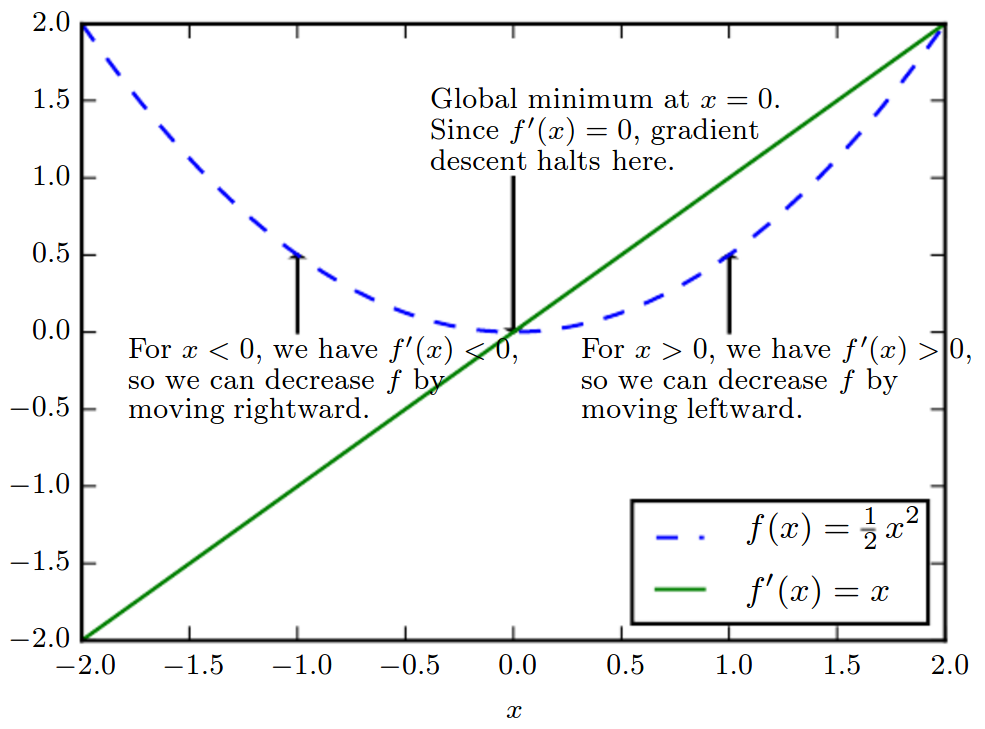
\includegraphics[width=10cm]{gambar/landasan-teori/gradient-descent.png}
    \caption{\textit{Gradient descent} menggunakan derivatif untuk meminimalkan sebuah fungsi \Parencite{Goodfellow-2016}}.
    \label{gambar:gradient-descent}
\end{figure}

Ketika \textit{feedforward neural network} menerima input $\pmb{x}$ dan menghasilkan output $\pmb{\hat{y}}$, informasi mengalir maju melalui jaringan. Input $\pmb{x}$ menyediakan informasi awal yang merambat ke \textit{hidden unit} pada setiap layer hingga akhirnya menghasilkan $\pmb{\hat{y}}$. Proses ini disebut \textit{forward propagation}. Dalam proses latihan, \textit{forward propagation} dapat terus maju sampai menghasilkan nilai skalar \textit{cost} $J(\theta)$. Algoritma \textit{backpropagation} memungkinkan informasi dari \textit{cost} mengalir mundur melalui jaringan untuk menghitung gradiennya. Gradien tersebut dihitung dengan mencari derivatif $\nabla_x J(\theta)$ dengan aturan rantai kalkulus \Parencite{Goodfellow-2016}.

Pada RNN, aktivasi \textit{hidden layer} tidak hanya mempengaruhi \textit{loss function} pada \textit{output layer}, namun juga mempengaruhi \textit{hidden layer} pada langkah waktu selanjutnya. Maka, gradien dihitung dengan menggunakan \textit{backpropagation} pada graf yang telah dibentangkan. Metode ini bernama \textit{Backpropagation Through Time (BPTT)} \Parencite{graves-2012}.

%------------------------------------------------------------------------------
% Pencarian Hyperparameter
%------------------------------------------------------------------------------
\section{Pemilihan \textit{Hyperparameter}}
Hyperparameter adalah pengaturan dalam algoritme pembelajara mesin yang perlu ditentuan di luar algoritme pembelajaran itu sendiri. Beberapa \textit{hyperparameter} berpengaruh pada waktu dan memori yang dibutuhkan untuk menjalanakan algoritme pembelajaran, sedangkan beberapa \textit{hyperparameter} lain mempengaruhi kemampuan model untuk memprediksi dengan tepat \Parencite{Goodfellow-2016}.

Beberapa metode yang populer untuk memilih \textit{hyperparameter} secara otomatis adalah \textit{grid search} dan \textit{random search}. Pada \textit{grid search}, variasi hyperparameter dipilih dari himpunan nilai yang akan diuji, lalu algoritme \textit{grid search} akan menguji setiap kombinasi nilai-nilai \textit{hyperparameter} tersebut. Pada \textit{random search}, algoritme menguji variasi \textit{hyperparameter} yang nilainya diambil secara acak dari sebuah distribusi marginal. Dibandingkan dengan \textit{grid search}, algoritme \textit{random search} dapat menghasilkan model yang sama baiknya atau lebih baik dengan waktu komputasi yang lebih singkat \Parencite{bergstra-2015}.

%------------------------------------------------------------------------------
% Tensorflow
%------------------------------------------------------------------------------
\section{TensorFlow}
TensorFlow adalah pustaka sumber terbuka pembalajaran mesin. TensorFlow melakukan komputasi yang dideskripsikan dengan model aliran data dan memetakannya ke berbagai jenis perangkat keras berbeda, mulai dari melakukan pengambilan kesimpulan pada perangkat bergerak seperti Android dan iOS, pelatihan dan sistem pengambilan keputusan berukuran sedang menggunakan satu mesin yang terdiri dari satu atau lebih kartu GPU sampai ke sistem pelatihan berskala besar yang berjalan pada ratusan mesin khusus dengan ribuan GPU \Parencite{abadi-2015}.

Graf aliran data dalam TensorFlow mendeskripsikan komputasi matematis dengan graf \textit{node} dan \textit{edge} terarah. \textit{Edge} memuat array multidimensi berukuran dinamis yang disebut dengan tensor. Para \textit{node} bekerja secara asinkron dan paralel ketika seluruh tensor pada \textit{edge} yang masuk telah tersedia. Aliran data tersebut direpresentasikan oleh TensorFlow melalui API yang tersedia untuk bahasa Python, C++, Java dan Go.
